\documentclass[12pt]{article}

\usepackage{packages/sbc/sbc-template}
\usepackage{graphicx,url}
\usepackage[utf8]{inputenc}
\usepackage[english]{babel}


\sloppy

\title{Code retrieval task analysis}

\author{Henrique Krausbug Correa\inst{1}, Viviane Pereira Moreira\inst{1}, Dennis Giovani Balreira\inst{1}}


\address{Instituto de Informática -- Universidade Federal do Rio Grande do Sul
  (UFRGS)\\
  Caixa Postal 15.064 -- 91.501-970 -- Porto Alegre -- RS -- Brazil
  \email{\{henrique,viviane,dgbalreira\}@inf.ufrgs.br}
}

\begin{document} 

\maketitle


% ( 150 words approximately )
\begin{abstract}
  TODO
\end{abstract}
     
% \begin{resumo} 
%   TODO
% \end{resumo}

\section{Introduction}
% (1 page)

% Context: Why is code retrieval important in NLP? What is XCodeEval’s role?

% Motivation:
%  - XCodeEval NL-Code task benchmark reports a great accuracy for all languages, but D language has a lower accuracy.
%  - Authors statement: "We suspect that the limited availability of resources for D in both The Stack (Kocetkov et al., 2022) dataset (training corpora of StarEncoder) and our XCODEEVAL dataset could account for this discrepancy. Also, the presence of more hard negative candidates (i.e., very similar to a correct code) makes it a challenging task to identify similar codes."
%  - However, by checking TABLE 4, D dataset size is greater than other languages such as Perl and Ocaml, which have higher accuracy. 

% Research questions:
%   - What is the root cause analysis for D language lower accuracy on code retrieval tasks?
%   - Can this performance be improved based on NLP class topics and published articles related to this 

\section{Background}

% (1–2 pages)

% Terminilogy: Define key terms (e.g., code retrieval, dense passage retrieval).

% XCodeEval Benchmark: Tasks, dataset structure, and original paper’s setup.

% Dense Passage Retrieval (DPR): How it works, why it’s used for code retrieval.

XCodeEval Benchmark

The XCodeEval benchmark is designed to evaluate neural retrieval models in the context of programming tasks. It contains:

    A training dataset, comprising (query, positive code, negative code) triplets (Figure~\ref{fig:training}).


\begin{figure}[ht]
\centering
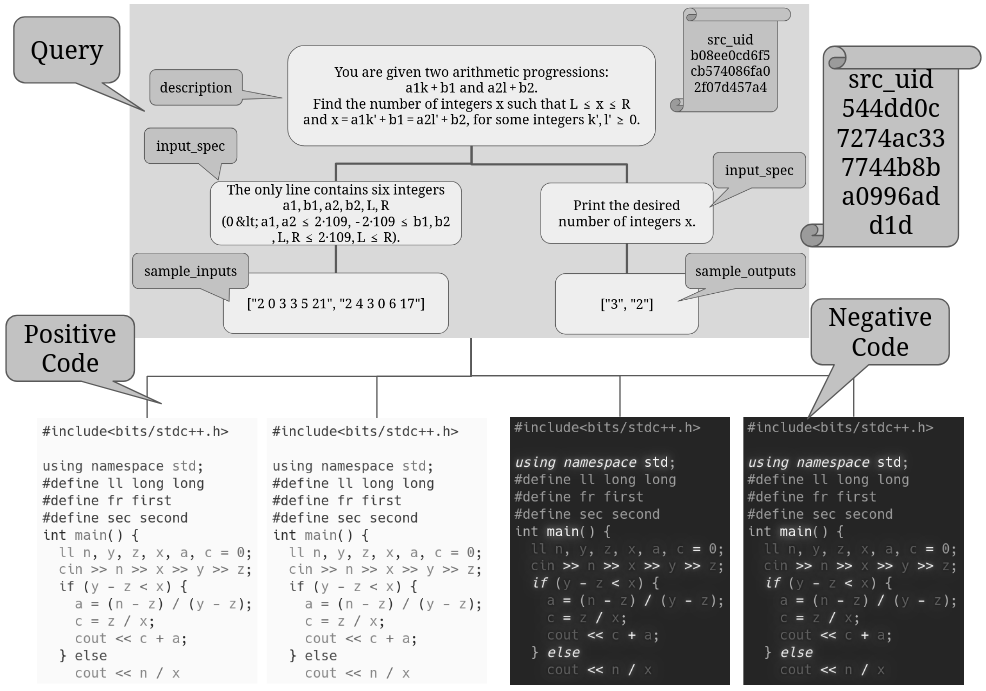
\includegraphics[width=1.0\textwidth]{images/task-gray.png}
\caption{Training dataset sample with query, positive and negative code}
\label{fig:training}
\end{figure}


\section{Related Work}

% (1–2 pages)

% Post Work: Summarize key papers on code retrieval that cite XCodeEval and criticize its limitations.

\section{Methodology}

%  (2–3 pages)

% Describe your approach to reproducing the XCodeEval benchmark.

% Data Preparation: How you processed XCodeEval (NL-Code template, corpus format).

% Model Setup:

%   DPR architecture (query/corpus encoders, multilingual training).

%   Hyperparameter (batch size, seq length, epochs) from the original paper.

% Evaluation Plan: Top-*k* accuracy (*k*=100), corpus/query embedding generation.

\section{Experimental Results}

% (3–4 pages)

% Describe framework, tools retrieval task results, and any preliminary findings.

% Expected vs. Actual: Compare original paper’s metrics to your observations.

% Possible Reasons for Divergence:

%   Training time insufficient? Hyperparameters not optimized?

%   Data preprocessing differences (e.g., template formatting).

% Qualitative Examples: Show some query-corpus pairs (even if not evaluated fully).

\section{Conclusion}

% (0.5 page)

% Lessons Learned: What would you do differently with more time/resources?

% Summary of efforts, challenges, and open questions.

% Alternative Approaches: Smaller models (e.g., ColBERT), approximate nearest-neighbor search (FAISS).

% Broader Implications: Reproducibility challenges in NLP research.

\bibliographystyle{packages/sbc/sbc}
\bibliography{paper}

\end{document}
